%
% Chapter 9
%
\chapter{Amplifier Revision Design}
The investigation of the first generation amp design and testing gave the team useful insight into what needed to change for the next hardware revision. An evaluation of the goals of Nessie2 provided the basis for the redesign. By exploring a number of hardware architecture choices we begin to rebuild the amplifier circuit from the beginning.
\section{Nessie2 Overview}
As capabilities of the CSEs and SLEDS arrays have increased, so too have requests from customers. What started as a project to drive a single 512x512 LED array has turned into a deep investigation to the physics and hardware constraints involved with increasing frame rates and resolutions. The eventual goal is a system able to drive a 2Kx2K array at 2kHz \cite{chris}.\par To move toward this new goal a distributed architecture using smaller CSEs was envisioned. Each CSE would be capable of driving twice as many analog channels on a quadrant of the new 2Kx2K array. The array would therefore be driven by four synchronized systems. To accomplish synchronization and analog integrity at this scale required a complete remodeling of the system firmware and hardware architecture. A prototype "Multi-CSE" system has been constructed as a proof-of-concept. In short, this system broke the Dewar pins out to routing boards that accepted all four cable outputs from a CSE each. Using the full bandwidth of a system greatly increased potential resolution and frame rate such that no system was driving more than a normal SLEDS array's worth of pixels. More details on the Multi-CSE prototype and Nessie2 architecture can be found in Christopher Jackson's doctoral dissertation \cite{chris}. The biggest change directly relevant to the analog design was that the main system would only output unamplified DAC signals along new coaxial cables to the Dewar. The Dewars main input board will contain cable receptacles and signal paths to mimic the old interface board. Included in this main input board will reside the new amplifiers. Moving this processing stage outside the system allowed us to consider many more functions for the amplifiers due to their proximity to the RIIC, which will be explored below.
\FloatBarrier
\begin{figure}[!htb]
	\centering
	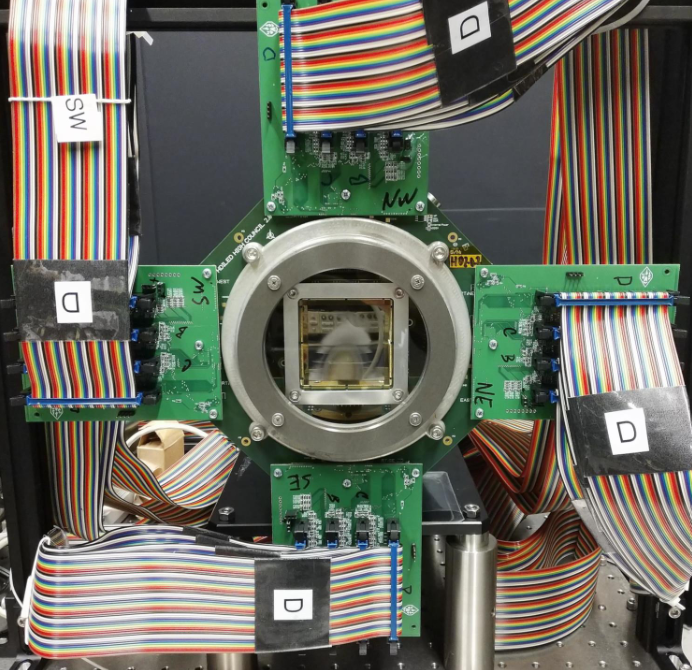
\includegraphics[]{multi_cse}
	\caption{Multi-CSE Prototype System}
\end{figure}

\begin{figure}[!htb]
	\centering
	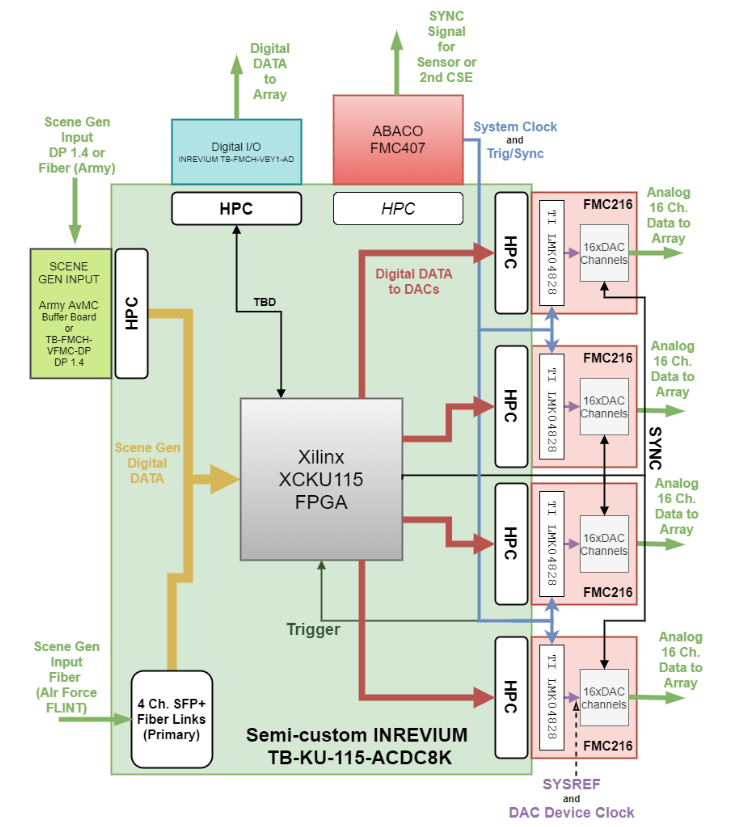
\includegraphics[]{nessie2_arch}
	\caption{Nessie2 System Architecture. Of note are the external ports for pre-amplified DAC output.}
\end{figure}

\FloatBarrier

\section{Objectives}
The goal of the new amplifiers is twofold. Due to the new increased resolution and frame rate, the system will have to be able to monitor and tune the amplifiers in order to maintain consistent output. In addition to producing the same level of signal quality from before, these cards had to have some level of analog analysis and response to appropriately self-tune. This is similar to the corrective role of the PC in creating NUC tables, but is system-level and intended to compensate for electrical differences in the large number of channels. An abstract architecture is as follows:
\begin{figure}[!htb]
	\centering
	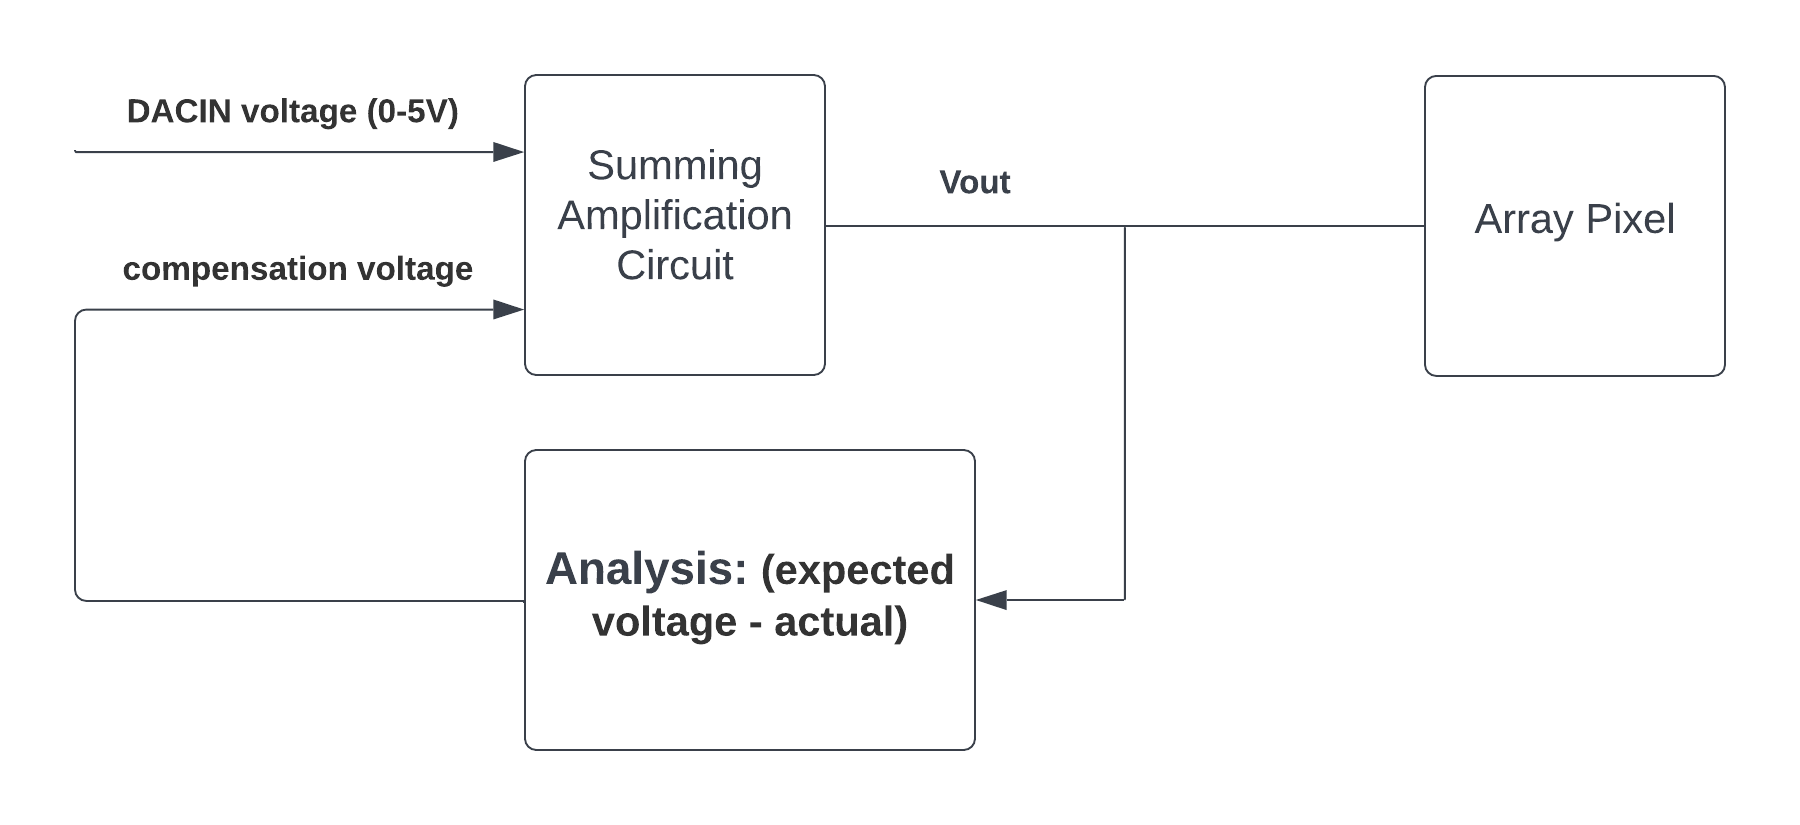
\includegraphics[]{amp2_block}
	\caption{Overview of the new analog component}
\end{figure}
\section{Amplifier Design Choices}
